\chapter{Exigences fonctionnelles}

\section{Portée du travail}

Le projet s'étend sur le terrain des logiciels orientés dans le coaching ainsi que des logiciels d'organisations de séance de sport individuel. Aujourd'hui, il existe beaucoup d'applications mobiles qui proposent des programmes statiques et qui ne tiennent pas compte de l'utilisateur. Or, les performances sportives dépendent grandement de la condition physique. D'autres applications sont juste des carnets de notes permettant à l'utilisateur de noter les exercices de sa séance. Cela lui permet juste d'avoir un suivi sur ses séances et c'est à l'utilisateur d'interpréter ces données.\\

Ces types d'applications ne conviennent donc pas aux personnes voulant débuter dans un sport et n'ayant aucune connaissance. Souvent ces types d'applications demandent une certaine expertise de l'utilisateur ou ne sont pas suffisamment complets pour permettre à une personne débutante de commencer un sport de manière autonome.   

\section{Portée du produit}

Notre application a pour objectif de permettre à son utilisateur de pouvoir débuter dans un sport individuel pour lequel il n'a pas de connaissance particulière. Toutefois, il pourrait moins convenir à un expert ou à quelqu'un pratiquant le sport depuis un moment puisqu'il possède déjà les connaissances nécessaire à la mise en oeuvre de son programme.\\

L'utilisateur pourra utiliser l'application pour établir des séances d'entrainement sur un sport individuel (natation, vélo, musculation, ...) et d'avoir un suivi automatique sur ses progrès dans ces séances. L'application pourra également lui convenir s'il cherche des conseils sur les salles de sport auxquelles se rendre pour faire ses séances.

\begin{figure}[!h]
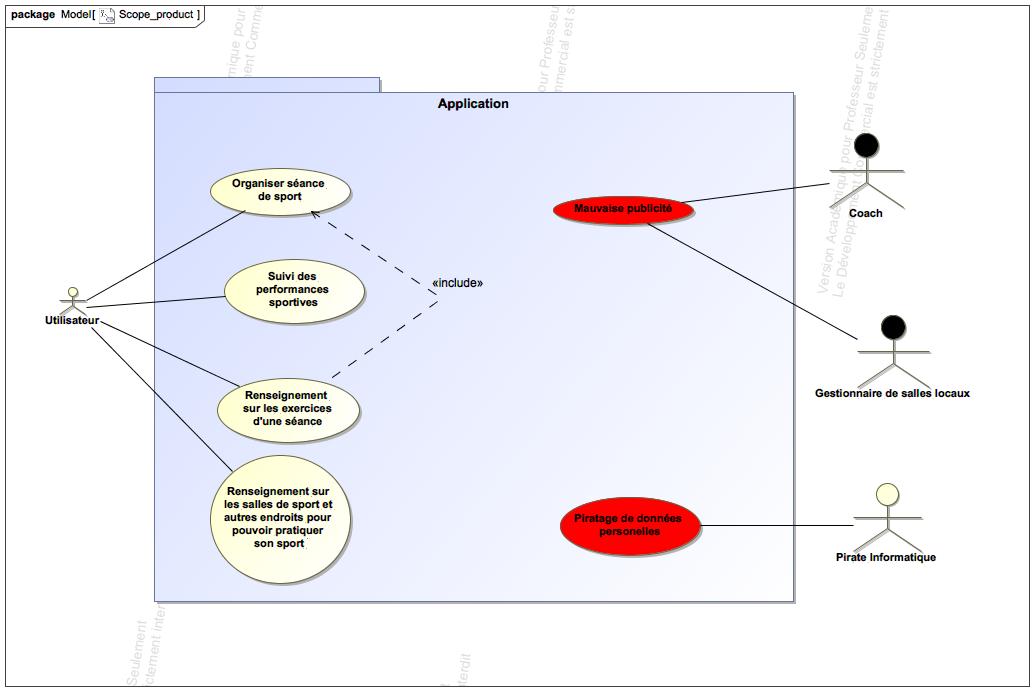
\includegraphics[scale=0.3]{diagrams/scope_product}
\centering
\hskip2em
\caption{Diagramme des cas d'utilisations du produit}
\end{figure}


\section{Description des exigences fonctionnelles}

\subsection*{Inscription dans le système}

L'utilisateur doit pouvoir s'inscrire à l'aide d'un formulaire en rentrant ses données personnelles telles que son nom, prénom, adresse email, mot de passe ou alors à l'aide de son compte Google ou Facebook. Une fois ses données personnelles enregistrées, il devra ensuite entrer ses propres caractéristiques physique comme son poids et sa taille. Il devra également indiquer ses objectifs en choisissant parmi une liste d'objectifs proposée par l'application.

\begin{figure}[!h]
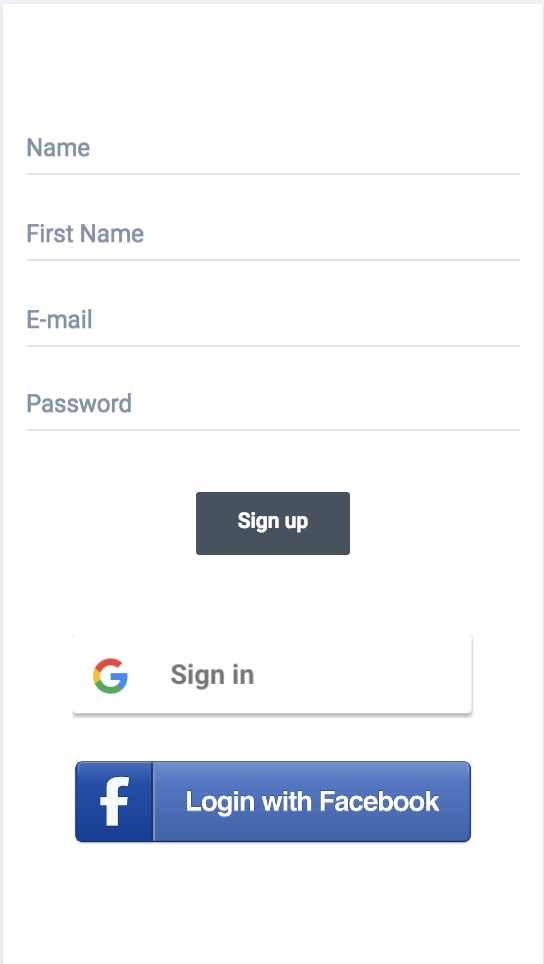
\includegraphics[scale=0.3]{ihms/inscription}
\centering
\hskip2em
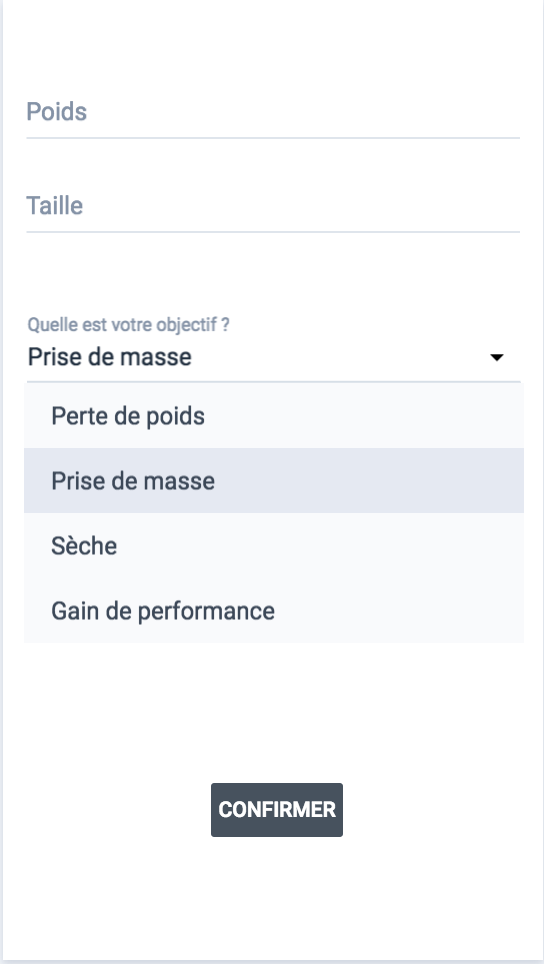
\includegraphics[scale=0.3]{ihms/caracteristiques}
\caption{Interfaces d'inscription}
\end{figure}


\begin{itshape}
User story : En tant qu'utilisateur, je veux rentrer mes données et caractéristiques personnelles dans le système pour m'inscrire.
\end{itshape}

\begin{figure}[!h]
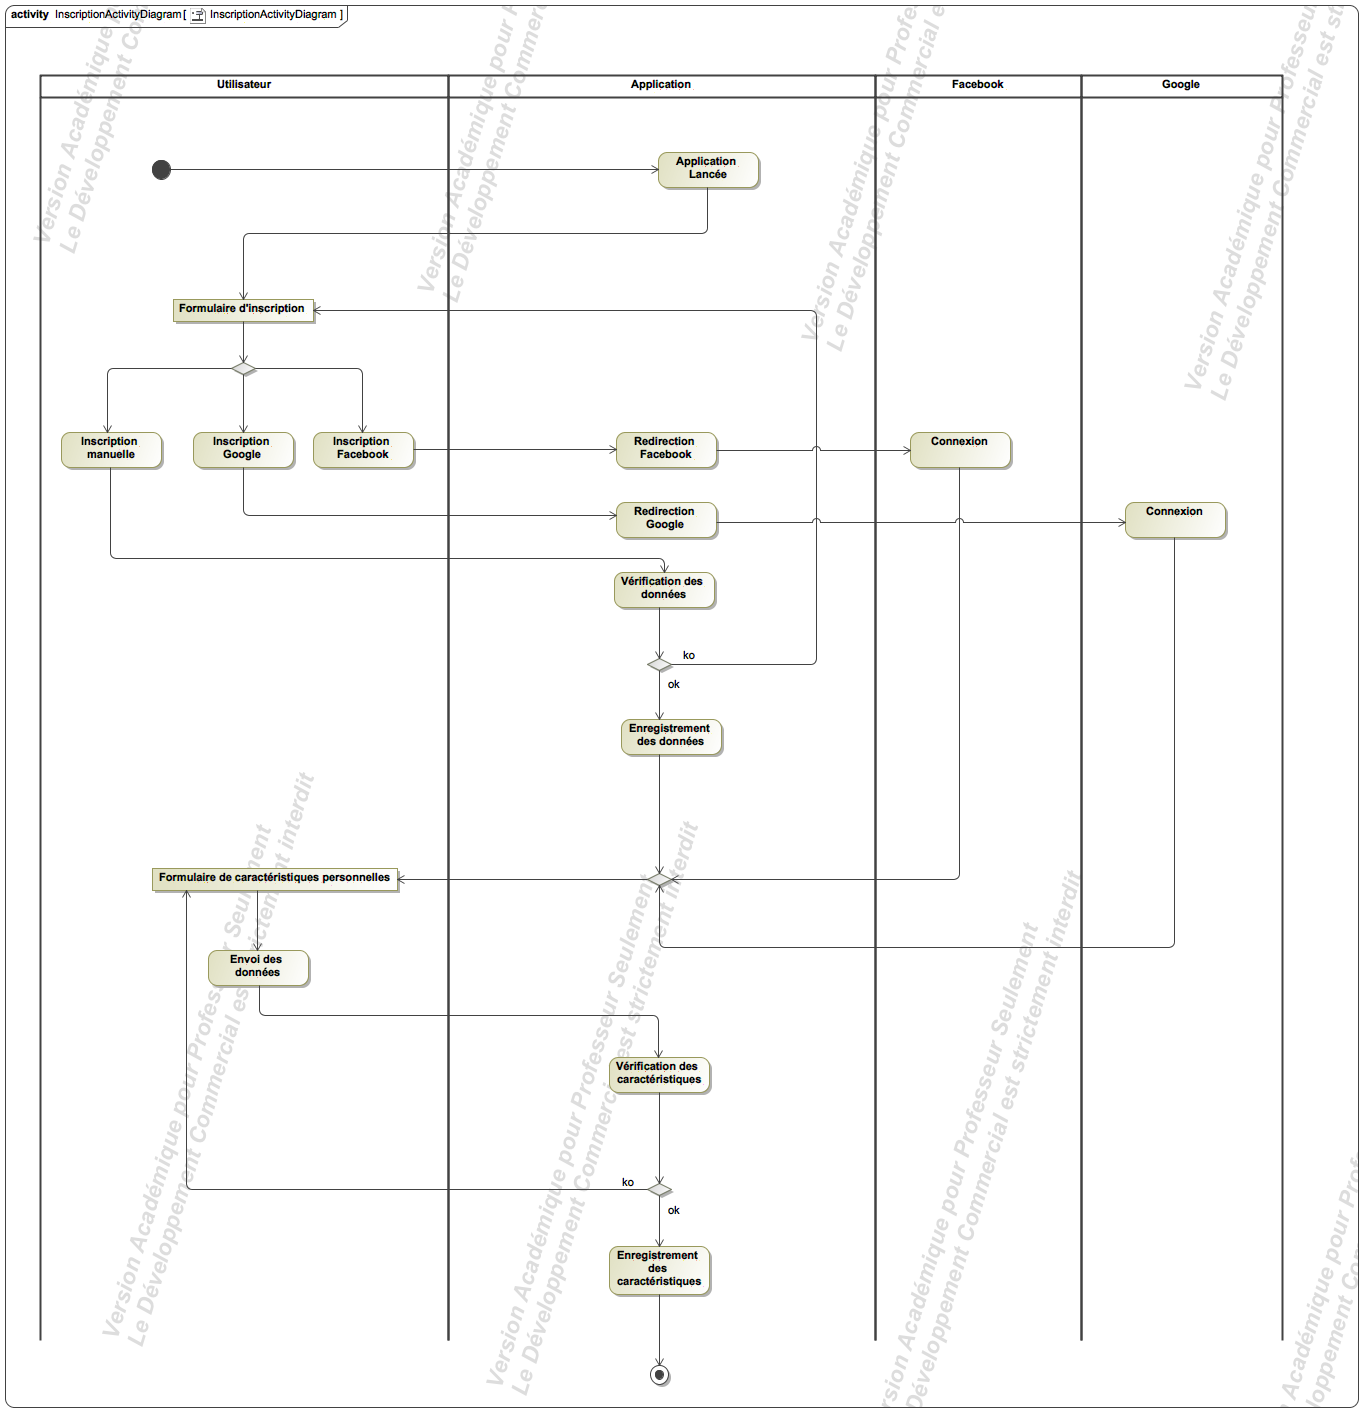
\includegraphics[scale=0.3]{diagrams/inscription}
\centering
\caption{Diagramme d'activité d'une inscription}
\end{figure}

\subsection*{Didacticiel}

Lorsque le scénario d'inscription est terminé, une séance est générée automatiquement au client selon son type de sport choisi. L'application lui proposera de cliquer sur tous les boutons disponibles, étapes par étapes à l'aide d'indications afin de bien prendre en main l'application. Une fois la séance terminée, l'utilisateur reçoit un badge pour avoir effectué sa toute première séance.\\


\begin{itshape}

User stories :

\begin{itemize}
\item En tant qu'utilisateur, je veux prendre l'application en main pour pouvoir l'utiliser à bon escient par la suite.
\item En tant que système, je propose un didacticiel à l'utilisateur pour que celui-ci utilise l'application correctement.
\end{itemize}

\end{itshape}

\subsection*{Utilisation normale (en séance)}
L'utilisateur, avant de pouvoir générer une séance de sport, doit préciser le sport, l'intensité et le temps à consacrer pour sa séance. Le formulaire qu'il devra compléter sera pré-remplie en fonction des choix de ses séances précédentes.   

\begin{figure}[!h]
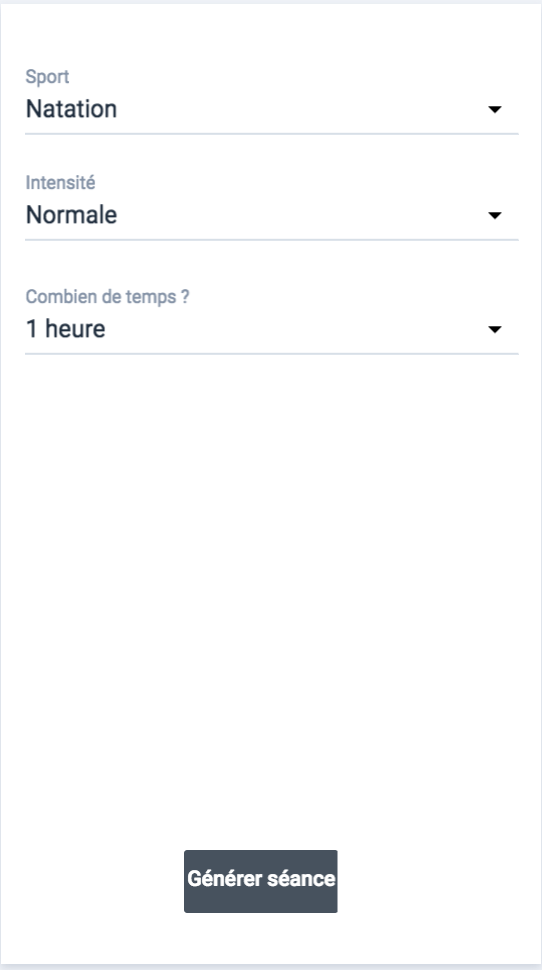
\includegraphics[scale=0.3]{ihms/seance}
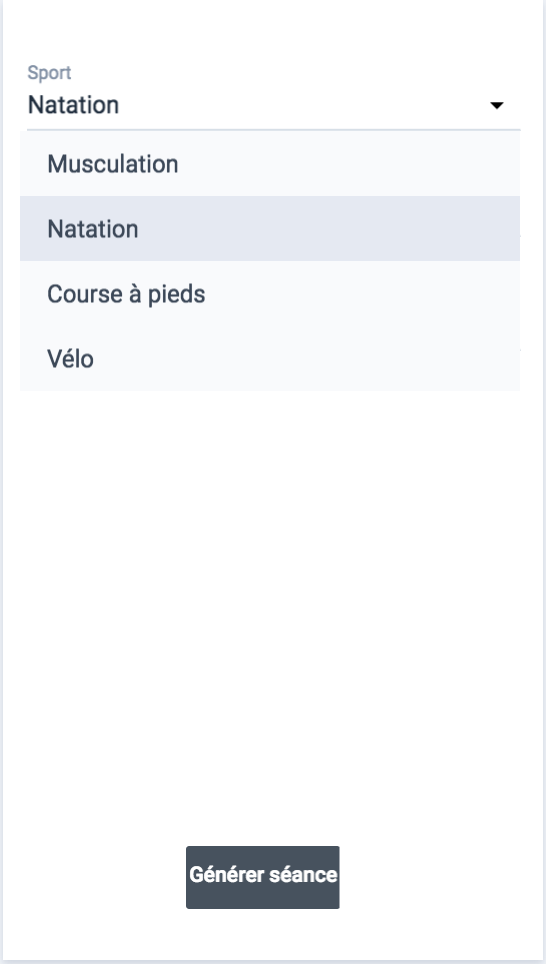
\includegraphics[scale=0.3]{ihms/seance2}
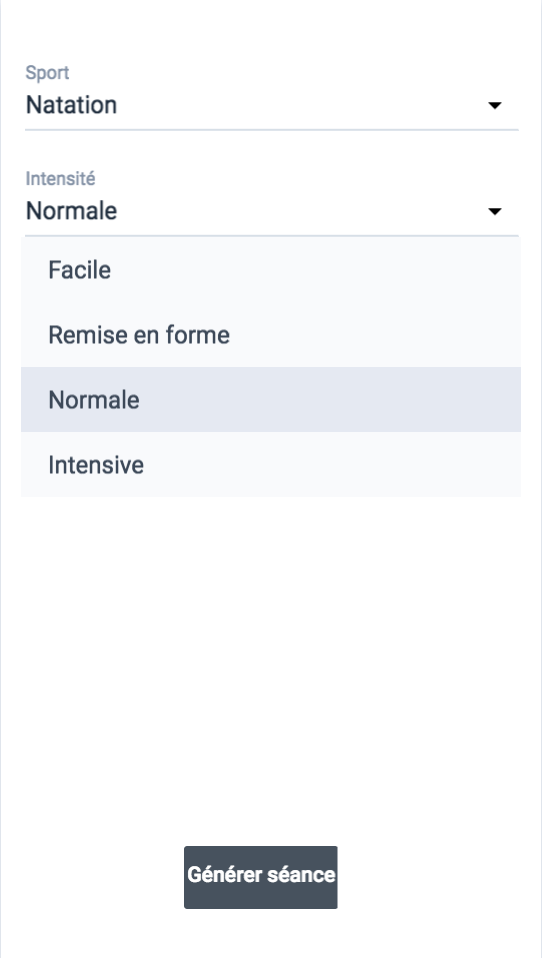
\includegraphics[scale=0.3]{ihms/seance3}
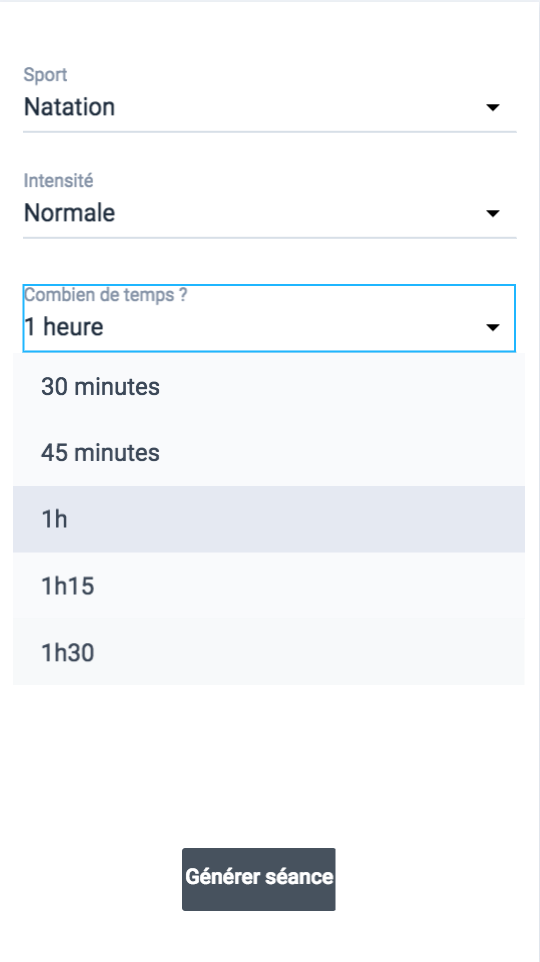
\includegraphics[scale=0.3]{ihms/seance4}
\centering
\caption{Interface de préparation de la séance}
\end{figure}

Une fois qu'il a confirmé ces informations, la séance est généré en fournissant à l'utilisateur une liste d'exercice à faire. Pour chaque exercice proposé, l'utilisateur pourra cliquer sur un sigle "Help" afin d'en savoir davantage sur l'exercice à réaliser. Ces informations d'aide peuvent être de types différents (vidéos, illustrations, textes). Une fois que l'utilisateur a fini tous les exercices, il doit valider sa séance en appuyant sur un bouton prévue à cet effet.\\ 

\begin{figure}[!h]
\centering
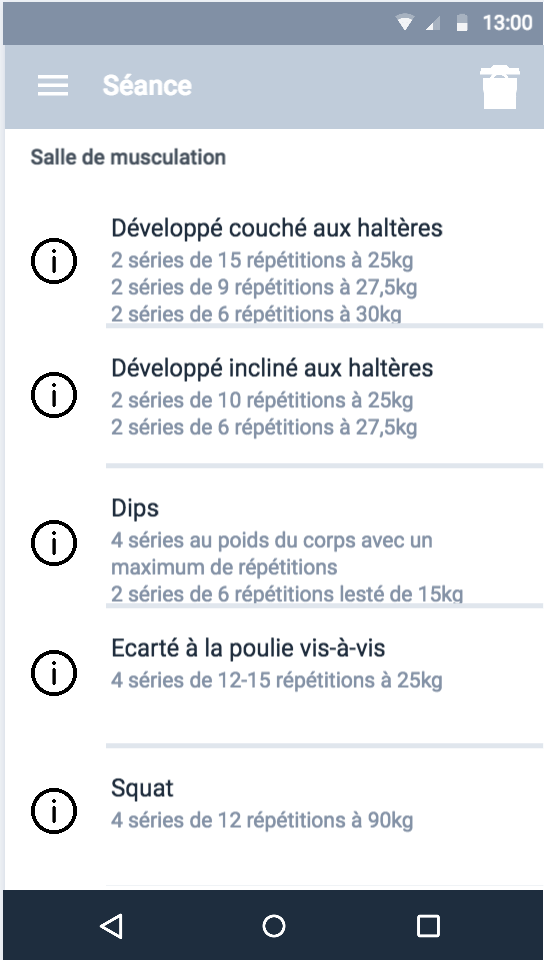
\includegraphics[scale=0.3]{ihms/normal_session}
\hskip2em
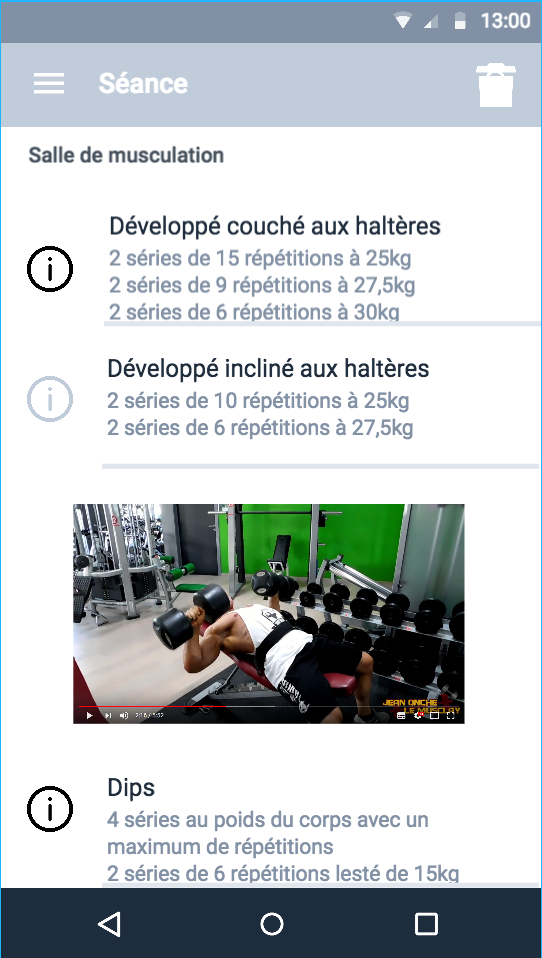
\includegraphics[scale=0.3]{ihms/get_information_about_exo}
\caption{Interface de la séance}
\end{figure}

\begin{itshape}
User story : En tant qu'utilisateur, j'attribue une cotation pour chacun des critères proposés pour améliorer le système dans sa globalité et le contenu des futures séances.

\end{itshape}

\newpage

\begin{figure}[!h]
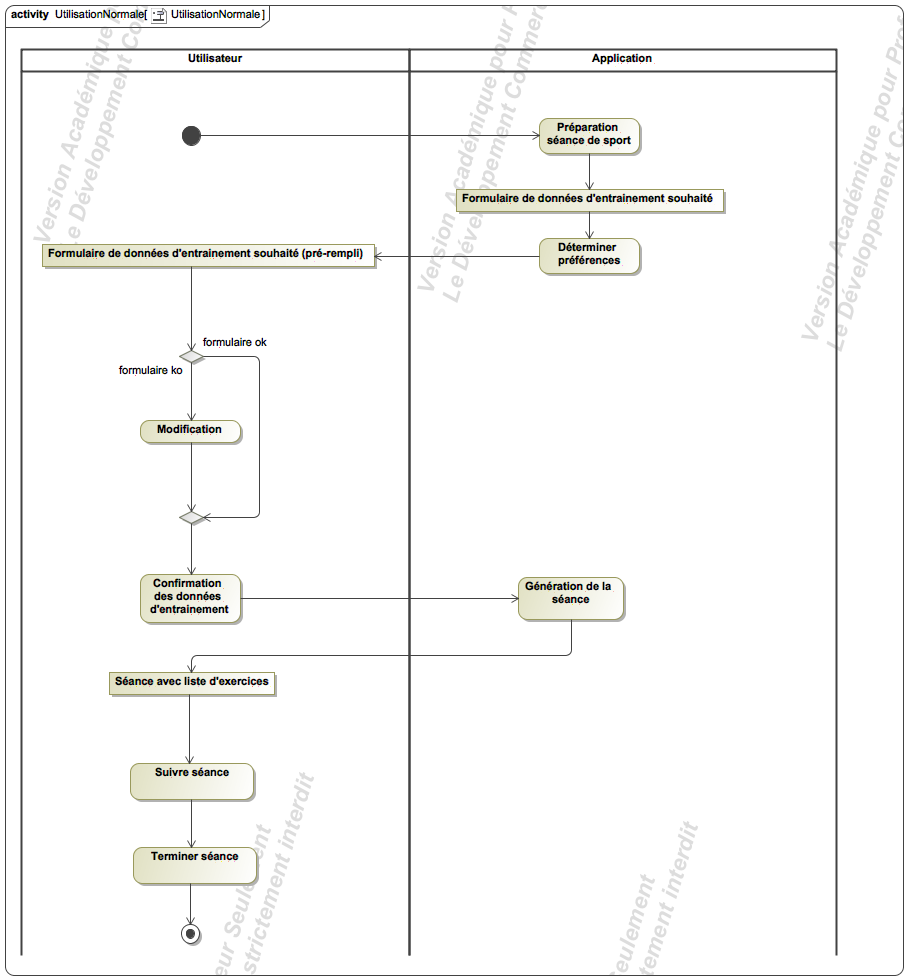
\includegraphics[scale=0.3]{diagrams/utilisation}
\centering
\caption{Diagramme d'activité d'une utilisation normale}
\end{figure}


\subsection*{Mise à jour des données (post-séance)}

Une fois la séance terminée et validée par l'utilisateur, les données d'entrainement sont mises à jour à l'aide de plusieurs critères tels que l'impression générale, la difficulté, ou si la durée de l'entrainement a été respectée. Chaque critère est côté sur base d'une note sur 5 donnée par l'utilisateur. Dès que l'utilisateur a validé toutes ses notes, il peut les confirmer et retourner sur l'écran d'accueil. L'application lui affiche un compteur de temps jusqu'à la prochaine séance "conseillée". Celui-ci reçoit un badge toutes les 10 séances respectées et sa barre de progression est mise à jour.  

\begin{figure}[!h]
\centering
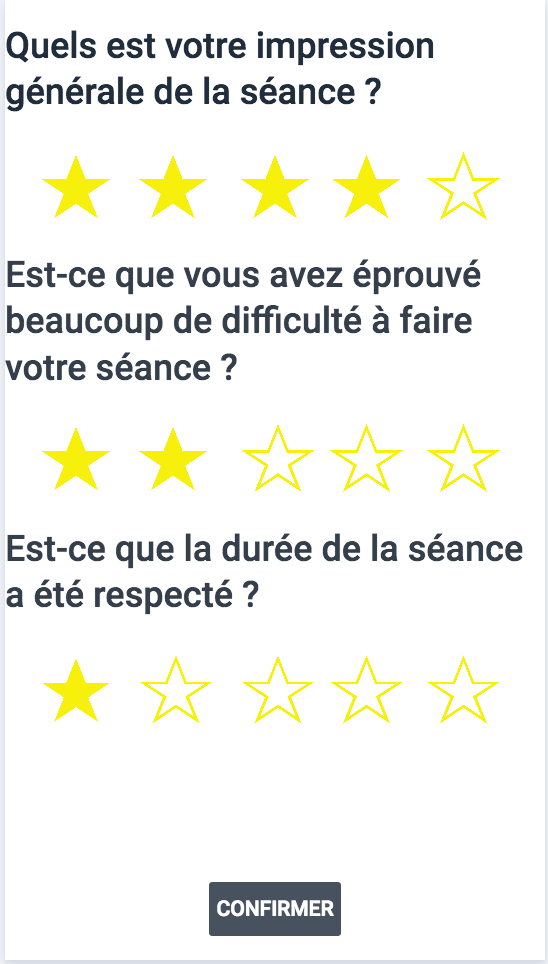
\includegraphics[scale=0.3]{ihms/rating_before_update}
\caption{Interface de mise à jour des données post-séance}
\end{figure} 

\begin{itshape}
En tant qu'utilisateur, j'attribue une cotation pour chacun des critères proposés pour améliorer le système dans sa globalité et le contenu des futures séances.
\end{itshape}

\begin{figure}[!h]
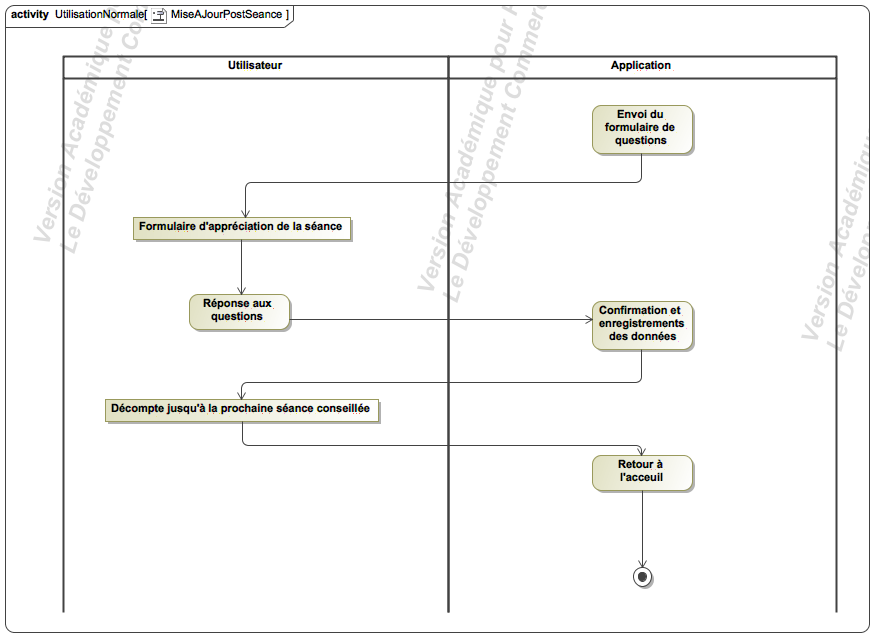
\includegraphics[scale=0.3]{diagrams/post}
\centering
\caption{Diagramme d'activité d'une mise à jour des données en post-séance}
\end{figure}

\subsection*{Suppression d'exercices d'une séance}

Lors de la génération de la séance, l'utilisateur peut cliquer sur une molette qui permettra de supprimer des exercices. Dans ce cas, une icône apparaît à côté de chaque exercice. Lorsqu'il clique dessus, il peut justifier son choix afin que l'exercice revienne dans les futures séances d'entrainements, ou non.

\begin{figure}[!h]
\centering
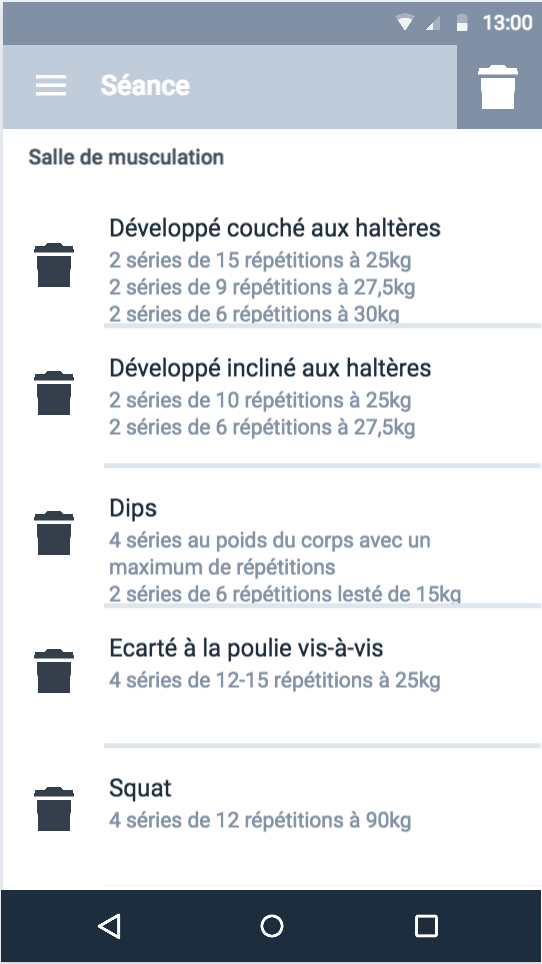
\includegraphics[scale=0.3]{ihms/remove_exo}
\caption{Suppression exercice}
\end{figure}

\begin{itshape}
User story : En tant qu'utilisateur, je choisis de supprimer des exercices inintéressants pour m'offrir une séance optimale et donner un feedback pour la suite de ces séances.
\end{itshape}

\subsection*{Recherche d'un complexe sportif par un utilisateur}

L'utilisateur doit pouvoir sélectionner son sport, et selon sa localisation, l'application lui propose le complexe sportif adéquat à proximité. En cliquant dessus, quelques infos seront données, comme la fréquentation, le matériel mis à disposition?\\

\begin{itshape}
User story : En tant que système, je propose à l'utilisateur les complexes sportifs les plus proches correspondant aux exigences et à la localisation de celui-ci pour que l'utilisateur soit conseillé de la meilleure des manières.

\end{itshape}


\subsection*{Les données d'entrainements et l'algorithme de préparation de séance}

Les séances d'un utilisateur doivent être organisées de façon dynamique en fonction des séances précédentes. Ceci nécessite donc que les séances soit préparés sur base d'un algorithme de \textit{machine learning} afin d'optimiser les performances de l'utilisateur et de proposer la meilleure séance possible permettant cette optimisation.\\

Plusieurs données seront également nécessaires pour la bonne réalisation des algorithmes de préparation de séance. D'une part, il est nécessaire d'entretenir des données d'entrainements pour l'utilisateur afin de déterminer au mieux comment organiser sa séance. Toutefois, ces données ne suffiront pas pour les algorithmes et auront besoin de grandes quantités de données afin de déterminer un modèle plus général sur base duquel interpréter les données d'entrainement de l'utilisateur.  